\documentclass[10pt]{article}
\usepackage[utf8]{inputenc}
\usepackage[T1]{fontenc}
\usepackage{amsmath}
\usepackage{amsfonts}
\usepackage{amssymb}
\usepackage[version=4]{mhchem}
\usepackage{stmaryrd}
\usepackage{graphicx}
\usepackage[export]{adjustbox}
\graphicspath{ {./images/} }

\begin{document}
\begin{enumerate}
  \item The graph below shows the velocity $v$ in metres per second of a particle at time $t$ seconds.\\
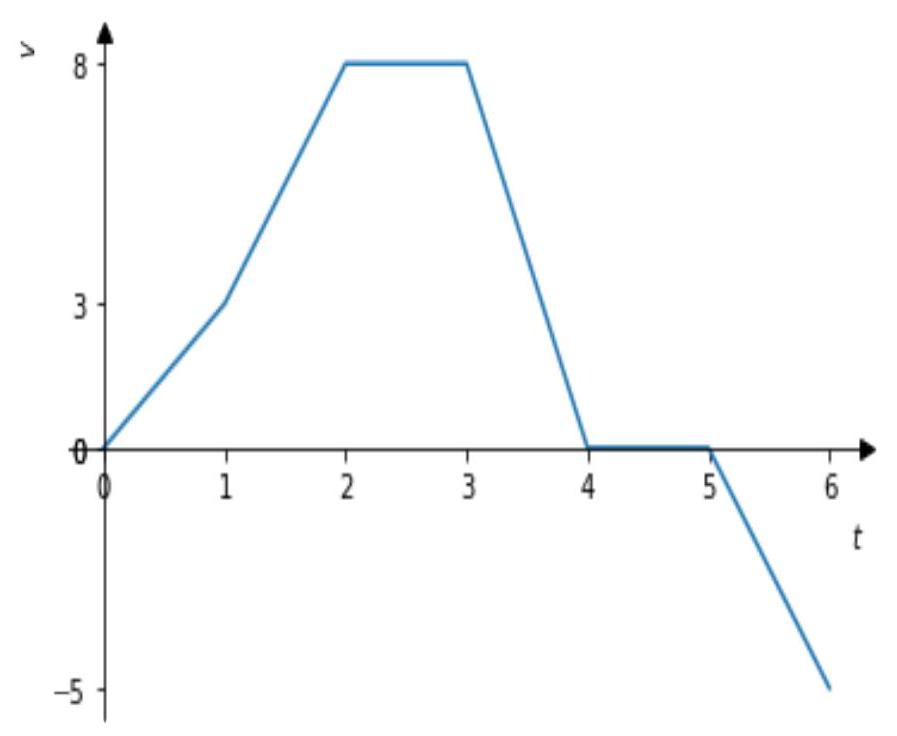
\includegraphics[max width=\textwidth, center]{2024_12_26_f16b160c9a5a429665deg-1}\\
(a) Describe the motion of this particle. When is it moving forwards? When is it accelerating? When is it decelerating?\\
(b) Express the velocity $v(t)$ as a function of $t$.\\
(c) Sketch a graph of the acceleration of this particle.\\
(d) Express the acceleration $a(t)$ of the particle as a function of $t$\\
(e) Sketch a graph for the position of this particle.\\
(f) Express the position $s(t)$ as a function of $t$
\end{enumerate}

\section*{Solution}
(a) The particle starts accelerating forward at a constant rate between $t=0$ and $t=1$, it then increases its acceleration until $t=2$. Between $t=2$ and $t=3$, it moves forward at a constant speed, and then begins to decelerate and reaches a stop at $t=4$ and stays still until $t=5$, at which point it starts accelerating backwards.\\
(b) We will show the first few line segments here. For $0 \leq t \leq 1$ we need to find the equation of the line going through the points $(0,0)$ and $(1,3)$. This is $v=3 t$, therefore $v(t)=3 t$. Then for $1 \leq t \leq 2$ we need to find the equation of the line through $(1,3)$ and $(2,8)$. This is $v=5 t-2$. We keep going like this to get the final answer

$$
v(t)= \begin{cases}3 t & 0 \leq t \leq 1 \\ 5 t-2 & 1 \leq t \leq 2 \\ 8 & 2 \leq t \leq 3 \\ -8 t+32 & 3 \leq t \leq 4 \\ 0 & 4 \leq t \leq 5 \\ -5 t+25 & 5 \leq t \leq 6\end{cases}
$$

(c)\\
(d) We can find the acceleration by differentiating the velocity. So we get

$$
a(t)= \begin{cases}3 & 0 \leq t \leq 1 \\ 5 & 1 \leq t \leq 2 \\ 0 & 2 \leq t \leq 3 \\ -8 & 3 \leq t \leq 4 \\ 0 & 4 \leq t \leq 5 \\ -5 & 5 \leq t \leq 6\end{cases}
$$

(e)\\
(f) Remember that velocity is the rate of change of position. This means that

$$
\frac{d}{d t} s(t)=v(t)
$$

So we need to find a function whose derivative is $v(t)$. This is the antiderivative of $v(t)$. For the interval $0 \leq t \leq 1$ we need to find some function whose derivative is $3 t$. Such a function is exactly of the form $\frac{3}{2} t^{2}+C$ where $C$ is some constant. We want our particle to start at distance 0 . So that means $s(0)=0$, so we need to choose $C=0$. This means that between 0 and 1 the distance is

$$
s(t)=\frac{3}{2} t^{2}
$$

So at $t=1$, the position of the particle is $\frac{3}{2}$. Between 1 and 2 we want the derivative to be $5 t-2$ and we also want $s(1)=\frac{3}{2}$. The antiderivative of $5 t-2$ is $\frac{5}{2} t^{2}-2 t+C$ where $C$ is some constant. By plugging in $t=1$, we see that $C$ has to equal 1. So between 1 and 2 the position is given by

$$
s(t)=\frac{5}{2} t^{2}-2 t+1
$$

So at $t=2$ the position is 7 . We keep going with the same method. The final answer should be.

$$
s(t)= \begin{cases}\frac{3}{2} t^{2} & 0 \leq t \leq 1 \\ \frac{5}{2} t^{2}-2 t+1 & 1 \leq t \leq 2 \\ 8 t-9 & 2 \leq t \leq 3 \\ -4 t^{2}+32 t-45 & 3 \leq t \leq 4 \\ 19 & 4 \leq t \leq 5 \\ -\frac{5}{2} t^{2}+25 t-43.5 & 5 \leq t \leq 6\end{cases}
$$

\begin{enumerate}
  \setcounter{enumi}{1}
  \item Suppose we have a circle inscribed in a square.\\
(a) If the perimeter of the square is increasing at a rate of $10 \mathrm{~m} / \mathrm{s}$, at what rate is the circumference of the circle increasing?\\
(b) If the area of the circle is increasing at a rate of $10 \mathrm{~m}^{2} / \mathrm{s}$, at what rate is the diagonal of the square increasing when the area of the circle is $\pi$ ?
\end{enumerate}

\section*{Solution}
(a) If the side length of the square is $s$. Then the radius $r$ of the circle is $s / 2$. Now the perimeter $P$ of the square is $4 s$, and the circumference $C$ of the circle is $2 \pi r=\pi \cdot s$. Therefore we can see that $C=\frac{\pi}{4} P$. Now if we differentiate with respect to time $t$ on both sides we get

$$
\frac{d C}{d t}=\frac{\pi}{4} \frac{d P}{d t}
$$

If the perimeter of the square is increasing at a rate of $10 \mathrm{~m} / \mathrm{s}$, then $\frac{d P}{d t}=10$, thefefore $\frac{d C}{d t}=2.5 \pi$\\
(b) The area of the circle $A$, is equal to $A=\pi r^{2}=\frac{\pi}{4} s^{2}$. The length of the diagonal of the square $D$ is equal to $D=\sqrt{2} s$. We want to write $D$ in terms of $A$. Notice that $\frac{\pi}{8} D^{2}=A$, therefore

$$
D=\frac{\sqrt{\pi}}{2 \sqrt{2}} \sqrt{A}
$$

So by differentiating both sides with respect to $t$ and using the chain rule we get

$$
\frac{d D}{d t}=\frac{\sqrt{\pi}}{2 \sqrt{2}} \frac{1}{2 \sqrt{A}} \cdot \frac{d A}{d t}
$$

The question wants us to evaluate this when $A=\pi$ and $\frac{d A}{d t}=10$. So we get the final answer is

$$
\frac{5}{2 \sqrt{2}}
$$

\begin{enumerate}
  \setcounter{enumi}{2}
  \item If $\$ 1500$ is borrowed at $8 \%$ interest, find the amounts due at the end of 5 years if the interest is compounded:\\
(a) annually;\\
(b) monthly;\\
(c) daily;\\
(d) continuously.
\end{enumerate}

\section*{Solution}
(a) The initial amount is 1500 . For each year we multiply it by 1.08 . So for 5 years this will be

$$
1.08^{5} \times 1500=2203.9921152
$$

(b) Now instead of multiplying by 1.08 for every year, we will multiply by

$$
\left(1+\frac{0.08}{12}\right)
$$

for every month. This means that the final amount due after 5 years is

$$
\left(1+\frac{0.08}{12}\right)^{12 \times 5} \times 1500=2234.76856245
$$

(c) Here we multiply by $\left(1+\frac{0.08}{365}\right)$ for every day, so the final amount due will be

$$
\left(1+\frac{0.08}{365}\right)^{365 \times 5} \times 1500=2237.63897036
$$

(d) Now we remember that the limit

$$
\lim _{n \rightarrow \infty}\left(1+\frac{0.08}{n}\right)^{n}=e^{0.08}
$$

Therefore, when the interest is compounded continuously, the final amount due is

$$
\left(e^{0.08}\right)^{5} \times 1500=2237.73704646
$$

\begin{enumerate}
  \setcounter{enumi}{3}
  \item Recall that the rate of cooling of an object is proportional to the difference in temperature between the object and its surrounding.\\
A freshly brewed cup of coffee has temperature $95^{\circ} \mathrm{C}$ in a $20^{\circ} \mathrm{C}$ room. When its temperature is $70^{\circ} \mathrm{C}$, it is cooling at a rate of $1^{\circ} \mathrm{C}$ per minute. When does this occur?
\end{enumerate}

\section*{Solution}
Since the rate of cooling of an object is proportional to the difference in temperature between the object and its surrounding, if we let $T$ denote the temperature of the cup and $t$ denote the time, then

$$
\frac{d T}{d t}=k(T-20)
$$

where $k$ is some constant. Now let $y=T-20$, then $\frac{d y}{d t}=\frac{d T}{d t}$. We can then write the equation above as

$$
\frac{d y}{d t}=k y
$$

This means that

$$
y=y_{0} e^{k t}
$$

where $y_{0}$ is the initial value for $y$. From the problem we can deduce that $y_{0}=95-20=$ 75. Therefore,

$$
y=75 e^{k t}
$$

and

$$
y^{\prime}=75 k e^{k t}
$$

The problem tells us that at a specific time $t_{0}$, we have $y\left(t_{0}\right)=70-20=50$ and $y^{\prime}\left(t_{0}\right)=-1$. Therefore

$$
50=75 e^{k t_{0}}
$$

and

$$
-1=75 k e^{k t_{0}}
$$

Dividing the two equations above, we get that $k=-\frac{1}{50}$. When we plug that back into our first equation we see that

$$
50=75 e^{-t_{0} / 50}
$$

We can rearrange this equation and take $\ln$ of both sides to find

$$
\ln (2 / 3)=-\frac{t_{0}}{50}
$$

Therefore,

$$
t_{0}=-50 \ln (2 / 3)=20.2732554054
$$

\begin{enumerate}
  \setcounter{enumi}{4}
  \item Two cars start moving from the same point. One travels south at $60 \mathrm{~km} / \mathrm{h}$ and the other travel west at $25 \mathrm{~km} / \mathrm{h}$. At what rate is the distance between the cars increasing two hours later?
\end{enumerate}

\section*{Solution}
The coordinates of the first care are $(0,-60 t)$, and the coordinates of the second one are $(-25 t, 0)$. So, the distance between the cars is

$$
\sqrt{25^{2} t^{2}+60^{2} t^{2}}=t \sqrt{25^{2}+60^{2}}=65 t
$$

So the distance between the cars is increasing at a constant rate of $65 \mathrm{~km} / \mathrm{h}$.\\
6. A particle is moving along the curve $y=\sqrt{x}$. As the particle passes through the point $(4,2)$, its $x$-coordinate increases at a rate of 3 units $/ \mathrm{s}$. How fast is its $y$-coordinate changing at this instant? Hint: think of the coordinates as functions of time, $y=y(t)$ and $x=x(t)$; what can you say about the coordinates of the particle at time $t$ ?.

\section*{Solution}
We can write $y, x$ as functions of $t$. So

$$
y(t)=\sqrt{x(t)}
$$

Differentiating both sides with respect to $t$ and using the chain rule we find

$$
y^{\prime}(t)=x^{\prime}(t) \frac{1}{2 \sqrt{x(t)}}
$$

We want to find $y^{\prime}$ when $x=4, y=2$ and $x^{\prime}=3$. So plugging these all in we find

$$
y^{\prime}=\frac{3}{2 \sqrt{4}}=\frac{3}{4} \mathrm{units} / \mathrm{s}
$$


\end{document}